\documentclass[12pt]{article}
\usepackage{preamble}

\pagestyle{fancy}
\fancyhead[LO,LE]{Теория вероятности}
\fancyhead[CO,CE]{19.11.2024}
\fancyhead[RO,RE]{Лекции Блаженова А. В.}

\fancyfoot[L]{\scriptsize исходники найдутся тут: \\ \url{https://github.com/pelmesh619/itmo_conspects} \Cat}

\begin{document}
    \section{Лекция 12}

    \hypertarget{jointdistribution}{}

    \subsection{Совместное распределение случайных величин}

    Пусть $\xi_1, \xi_2, \dots, \xi_n$ заданы на одном и том же вероятностном пространстве $(\Omega, \mathcal{F}, p)$

    \Def Случайным вектором $\vec{\xi} = (\xi_1, \xi_2, \dots, \xi_n)$ называется упорядоченный набор случайных величин, заданных
    на одном вероятностном пространстве

    Случайный вектор задает отображение $(\xi_1, \dots, \xi_n) (\omega) : \Omega \longrightarrow \Real^n$

    Поэтому случайный вектор еще называют многомерной случайной величиной, 
    а соответствующее ей распределение многомерным распределением: 

    $\forall B \in \mathcal{B}(\Real^n) \qquad P(B) = P(\omega \in \Omega \ | \ (\xi_1, \dots, \xi_n) \in B)$

    Таким образом, получили новое вероятностное пространство. В качестве элементарных исходов берем точки многомерного пространства, 
    а $\sigma$-алгебра - многомерное Борелевская $\sigma$-алгебра

    $(\Real^n, \mathcal{B}(\Real^n), P(B))$

    \hypertarget{jointdistributionfunction}{}

    \subsubsection{Функция распределения}

    \Def Функцией совместного распределения случайных величин $\xi_1, \xi_2, \dots, \xi_n$ называется функция 
    $F_{\xi_1, \xi_2, \dots, \xi_n}(x_1, x_2, \dots, x_n) = P(\xi_1 < x_1, \xi_2 < x_2, \dots, \xi_n < x_n)$

    \Notas Распределение полностью задается функцией распределения

    \Nota В дальнейшем, в основном, будем рассматривать системы из 2 случайных величин. Функция распределения в данном случае $F_{\xi, \eta}(x, y) = P(\xi < x, \eta < y)$ - вероятность попадания в эту область.

    \begin{center}
        \includegraphics[width=0.55\textwidth]{probtheory/images/probtheory_2024_11_19_1}
    \end{center}

    \hypertarget{jointdistributionfunctionproperties}{}

    \subsubsection{Свойства функции распределения}

    \begin{enumerate}
        \item $0 \leq F_{\xi, \eta}(x, y) \leq 1$
        \item $F_{\xi, \eta}(x, y)$ - неубывающая по каждому аргументу
        \item $\lim_{x \to -\infty} F_{\xi, \eta}(x, y) = \lim_{y \to -\infty} F_{\xi, \eta}(x, y) = 0, $
        $\lim_{\substack{x \to \infty \\ y \to \infty}} F_{\xi, \eta}(x, y) = 1$

        \item Восстановление маргинального (частного) распределения: 
        $\lim_{x \to \infty} F_{\xi, \eta}(x, y) = F_\eta(y)$, и наоборот - $\lim_{y \to \infty} F_{\xi, \eta}(x, y) = F_\xi(x)$

        \item $F_{\xi, \eta}(x, y)$ - непрерывна слева по каждому аргументу

        \item $P(x_1 \leq \xi < x_2, y_1 \leq \eta < y_2) = F_{\xi, \eta}(x_2, y_2) - F_{\xi, \eta}(x_2, y_1) - F_{\xi, \eta}(x_1, y_2) + F_{\xi, \eta}(x_1, y_1)$
    \end{enumerate}

    \hypertarget{randomvariablesindependence}{}

    \subsection{Независимость случайных величин}

    \Def Случайные величины $\xi_1, \dots, \xi_n$ независимы в совокупности, если для любого набора Борелевских множеств из
    $\mathcal{B}(\Real^n)$, $B_1, B_2, \dots, B_n$

    $p(\xi_1 \in B_1, \xi_2 \in B_2, \dots, \xi_n \in B_n) = p(\xi_1 \in B_1) \cdot p(\xi_2 \in B_2) \cdot \dots \cdot p(\xi_n \in B_n)$

    \Def Случайные величины $\xi_1, \xi_2, \dots, \xi_n$ попарно независимы, если независимы любые две из них

    \Notas Из независимости в совокупности следует попарная независимость: 

    $\xi_1, \dots, \xi_n$ независимы в совокупности, тогда покажем $\forall i, j \ \xi_i$ и $\xi_j$ - независимы

    Возьмем набор $B_i, B_j \in \mathcal{B}(\Real^n)$, при $k \neq i, j \ B_k = \Real$ \hfill $P(\xi_k \in B_k) = 1$

    Тогда $p(\xi_1 \in B_1, \dots, \xi_n \in B_n) = P(\xi_i \in B_i, \xi_j \in B_j) = P(\xi_i \in B_i) \cdot P(\xi_j \in B_j)$

    \Nota Из попарной независимости не следует независимость в совокупности, как видно из примера Берншейна

    Под независимыми величинами будем понимать независимые в совокупности

    \hypertarget{discretesystemoftwovariables}{}

    \subsection{Дискретная система двух случайных величин}

    \Def Случайные величины $\xi, \eta$ имеют совместное дискретное распределение, если случайный вектор $(\xi, \eta)$
    принимает не более, чем счетное число значений, то есть существует конечный или счетный набор пар чисел $(x_i, y_i)$, 
    таких что $P(\xi = x_i, \eta = y_i) > 0, \sum_{i, j} P(\xi = x_i, \eta = y_i) = 1$

    Таким образом двумерная дискретная случайная величина задается законом распределения - таблице вероятностей

    \begin{tabular}{c|c|c|c|c}
        $\xi \backslash \eta$ & $y_1$ & $y_2$ & $\dots$ & $y_m$ \\
        \hline
        $x_1$ & $p_{11}$ & $p_{12}$ & $\dots$ & $p_{1m}$ \\
        \hline
        $x_2$ & $p_{21}$ & $p_{22}$ & $\dots$ & $p_{2m}$ \\
        \hline
        $\vdots$ & $\vdots$ & $\vdots$ & $\ddots$ & $\vdots$ \\
        \hline
        $x_n$ & $p_{n1}$ & $p_{n2}$ & $\dots$ & $p_{nm}$ \\
    \end{tabular}

    Условие нормировки: $\sum_{i, j} p_{i, j} = 1$

    Зная общий закон распределения, можно восстановить частное (маргинальное) распределение по формулам: 

    $p_i = \sum_{j = 1}^m p_{i, j} \qquad q_j = \sum_{i = 1}^n p_{i, j}$

    \Def Дискретные случайные величины $\xi_1, \xi_2, \dots, \xi_n$ независимы, если для любых $x_1, x_2, \dots, x_n$ 
    $p(\xi_1 = x_1, \xi_2 = x_2, \dots, \xi_n = x_n) = p(\xi_1 = x_1) \cdot p(\xi_2 = x_2) \cdot \dots \cdot p(\xi_n = x_n)$

    При $n = 2$: $p_{i, j} = p_i \cdot q_j \ \forall i, j$

    \Ex

    \begin{tabular}{c|c|c|c|c}
        $\xi \backslash \eta$ & $-1$ & $0$ & $1$ & $p_i$ \\
        \hline
        $-1$ & $0.1$ & $0.2$ & $0.1$ & $0.4$ \\
        \hline
        $2$ & $0.2$ & $0.3$ & $0.1$ & $0.6$ \\
        \hline
        $q_j$ & $0.3$ & $0.5$ & $0.2$ & $\Sigma = 1$ \\
    \end{tabular}

    Найти маргинальное распределение и проверить независимость случайных величин


    \begin{tabular}{c|c|c}
        $\xi$ & $-1$ & $2$ \\
        \hline
        $p_i$ & $0.4$ & $0.6$  \\
    \end{tabular}

    \begin{tabular}{c|c|c|c}
        $\eta$ & $-1$ & $0$ & $1$ \\
        \hline
        $q_j$ & $0.3$ & $0.5$ & $0.2$  \\
    \end{tabular}

    $p_{11} = 0.1 \neq 0.12 = p_1 \cdot q_1 \qquad \Longrightarrow \xi, \eta$ - зависимы

    \hypertarget{continuoussystemoftwovariables}{}

    \subsection{Абсолютно непрерывная система двух случайных величин}

    \Def Случайные величины $\xi$ и $\eta$ имеют абсолютно непрерывное совместное распределение, если
    $\exists f_{\xi, \eta}(x, y)$, такая что $\forall B \in \mathcal{B}(\Real^2) \ P((\xi, \eta) \in B) = \iint_B f_{\xi, \eta}(x, y) dxdy$

    Функцию $f_{\xi, \eta}(x, y)$ будем называть функцией плотности совместного распределения случайных величин $\xi$ и $\eta$

    \underline{Геометрический смысл} плотности: 
    
    \begin{center}
        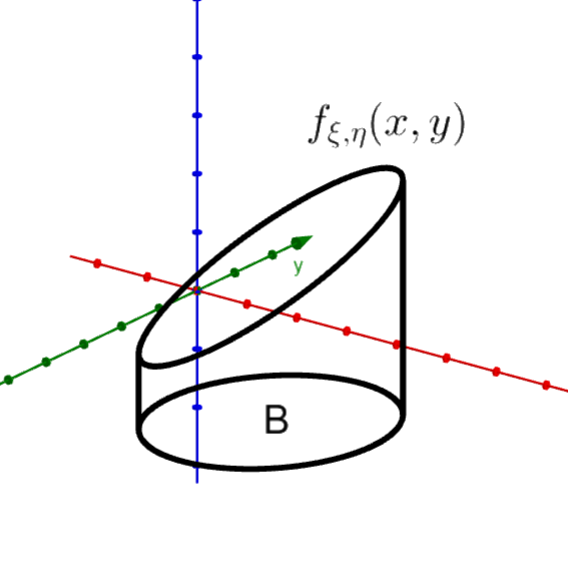
\includegraphics[width=0.55\textwidth]{probtheory/images/probtheory_2024_11_19_2}
    \end{center}

    \hypertarget{densityfunctionpropertiesincontinuoussystem}{}

    \underline{Свойства} плотности:

    \begin{enumerate}
        \item $f_{\xi, \eta}(x, y) \geq 0$
        \item Условие нормировки: $\iint_{\Real^2} f_{\xi, \eta}(x, y) dxdy = 1$
        \item $F_{\xi, \eta} = \int_{-\infty}^x \int_{-\infty}^y f_{\xi, \eta}(x, y) dydx$

        \item $f_{\xi, \eta}(x, y) = \frac{\partial^2 F_{\xi, \eta}(x, y)}{\partial x \partial y}$
        
        \item Если случайные величины $\xi, \eta$ имеют абсолютно непрерывное совместное распределение с плотностью $f(x, y)$, 
        то маргинальное распределение величин $\xi, \eta$ также имеют абсолютно непрерывное распределение
        с плотностями $f_\xi(x) = \int_{-\infty}^\infty f_{\xi, \eta}(x, y) dy, f_\eta(y) = \int_{-\infty}^\infty f_{\xi, \eta}(x, y) dx$

        \begin{MyProof}
            $F_{\xi}(x) = \lim_{y \to \infty} F_{\xi, \eta}(x, y) = \int_{-\infty}^x \int_{-\infty}^\infty f(x, y) dydx$

            Из этого $\int_{-\infty}^\infty f(x, y) dy = f_\xi(x)$
        \end{MyProof}

        \item Так как вероятность попадания в Борелевские множества полностью задается функцией распределения, 
        то условие независимости случайных величин эквивалентно следующему:

        $\xi_1, \xi_2, \dots, \xi_n$ независимы, если функция общего распределения распадается в произведение 
        отдельных функцию распределения
    
        $F_{\xi_1, \xi_2, \dots, \xi_n}(x_1, x_2, \dots, x_n) = F_{\xi_1}(x_1) \cdot F_{\xi_2}(x_2) \cdot \dots \cdot F_{\xi_n}(x_n)$

        \item \textit{Равносильное определение}: абсолютно непрерывные случайные величины $\xi_1, \dots, \xi_n$ независимы в совокупности тогда и только тогда, 
        когда плотность совместного распределения $f_{\xi_1, \xi_2, \dots, \xi_n}(x_1, x_2, \dots, x_n) = f_{\xi_1}(x_1) \cdot f_{\xi_2}(x_2) \cdot \dots \cdot f_{\xi_n}(x_n)$
    
        \begin{MyProof}
            При $n = 2$ случайные величины $\xi$ и $\eta$ независимы $\Longleftrightarrow F_{\xi, \eta}(x, y) = F_\xi(x) \cdot F_\eta(y) = \int_{-\infty}^x f_\xi(x) dx \cdot \int_{-\infty}^y f_\eta(y) dy = \int_{-\infty}^x \int_{-\infty}^y f_\xi(x) \cdot f_\eta(y) dxdy \Longrightarrow f_{\xi,\eta}(x, y) = f_\xi(x)f_\eta(y)$

            Аналогично для высших размерностей
        \end{MyProof}

    \end{enumerate}

    \Nota Совместное распределение абсолютно непрерывных случайных величин не обязано быть абсолютно непрерывным, оно может быть сингулярным

    \Exs Бросаем точку на отрезок прямой $y = x$ ($0 \leq x, y \leq 1$), $\xi$ - абсцисса точки, $\eta$ - ордината точки

    Случайный вектор $(\xi, \eta)$ имеют сингулярное распределение (непрерывное с нулевой областью) - 
    так как число элементарных исходов несчетно, но мера Лебега в $\Real^2$ отрезка равна 0

    \Nota Совместное распределение $\xi_1, \xi_2, \dots, \xi_n$ будет сингулярным, если одна из координат является функцией других (наблюдается функциональная зависимость)

    \subsection{Многомерное равномерное распределение}

    \Def $\letsymbol D \subset \Real^n$ - Борелевское множество в $\Real^n$ с конечной мерой Лебега ($0 < \lambda(D) < \infty$),
    случайный вектор $(\xi_1, \dots, \xi_n)$ имеет равномерное распределение, если плотность совместного распределения 
    постоянна в данной области и равна нулю вне данной области

    $f_{\xi_1, \dots, \xi_n}(x_1, \dots, \x_n) = \begin{cases}\frac{1}{\lambda(D)}, & \text{если } (x_1, \dots, x_n) \in D \\ 0, & \text{если } (x_1, \dots, x_n) \not\in D\end{cases}$


\end{document}
